\documentclass[12pt, twoside]{article}
\usepackage[letterpaper, margin=1in, head=30pt, headsep=0.1in]{geometry}
\usepackage[english]{babel}
\usepackage[utf8]{inputenc}
\usepackage{amsmath}
\usepackage{amsfonts}
\usepackage{amssymb}
\usepackage{tikz}
\usetikzlibrary{quotes, angles}

\usepackage{graphicx}
\usepackage{enumitem}
\usepackage{multicol}

%\usepackage{pgfplots}
%\pgfplotsset{width=10cm,compat=1.9}
%\usepgfplotslibrary{statistics}
%\usepackage{pgfplotstable}
%\usepackage{tkz-fct}
%\usepackage{venndiagram}

\usepackage{fancyhdr}
\pagestyle{fancy}
\fancyhf{}
\renewcommand{\headrulewidth}{0pt} % disable the underline of the header
\raggedbottom
\newif\ifmeta
\metatrue %print standards and topics tags

\title{Math AI Worksheet Generator and Formative Assessment System}
\author{Chris Huson}
\date{January 2021}

%\fancyhead[RE]{\thepage}
%\fancyhead[RO]{\thepage \\ Name: \hspace{3cm}}
%\fancyhead[L]{BECA / Dr. Huson / 10th Grade Geometry\\* 7 June 2019}
%
%\begin{document}
%\subsubsection*{13.7 Homework: Cross sections, distance applications}
%\fancyhead[L]{BECA / Dr. Huson / Geometry 03-Volume+angle-bisectors\\* pset ID: 34}

\begin{document}

\subsubsection*{5.11 Spicy: Transversals and parallel lines}
\begin{enumerate}

  \subsubsection*{Angle relationships}
  \item Review: Angle postulates and theorems you have learned. 
  \begin{enumerate}
    \item $\perp$ lines and complementary $\angle$s make $90^\circ$
    \item linear pairs add to $180^\circ$
    \item vertical $\angle$s are $\cong$
    \item definition of an angle bisector
    \item isosceles base angle theorem
  \end{enumerate}

\newpage
\item New theorems for parallel lines
  \begin{multicols}{2}
    \begin{enumerate}
      \item \emph{corresponding} $\angle$s of $\parallel$ lines are $\cong$\\
        $\angle 2 \cong \angle 6$
      \item \emph{same-side interior} $\angle$s are supplementary\\
      $m\angle 3 + m\angle 5 =  180$
      \item \emph{alternate exterior} $\angle$s are $\cong$\\
      $\angle 2 \cong \angle 7$
    \end{enumerate}
      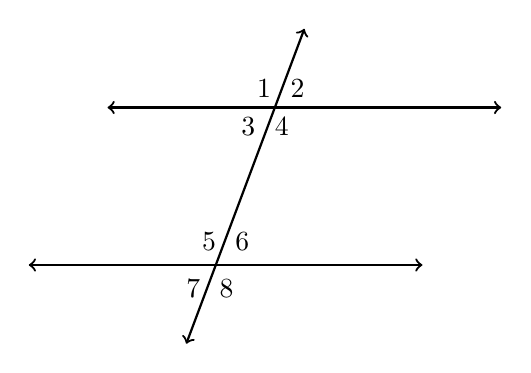
\begin{tikzpicture}[scale=1]
      \draw [<->, thick] (3,2)--(8,2);
      \draw [<->, thick] (2,0)--(7,0);
      \draw [<->, thick] (4,-1)--(5.5,3);
      \node at (4.5,0.3) [left]{$5$};
      \node at (4.5,0.3) [right]{$6$};
      \node at (4.3,-0.3) [left]{$7$};
      \node at (4.3,-0.3) [right]{$8$};
      \node at (5.2,2) [above left]{$1$};
      \node at (5.2,2) [above right]{$2$};
      \node at (5,2) [below left]{$3$};
      \node at (5,2) [below right]{$4$};
    \end{tikzpicture}
  \end{multicols}
  Hint: There are only two angle measures, the acute angles and the obtuse angles\\ (and they add to $180^\circ$)

\newpage
\item Given two parallel lines and a transversal, as shown, with $m\angle 6 =  70^\circ$. Write down the value of each angle measure.
  \begin{multicols}{3}
    \begin{enumerate}[itemsep=0.5cm]
      \item $m\angle 1 = $
      \item $m\angle 2 = $
      \item $m\angle 3 = $
      \item $m\angle 4 = $
      \item $m\angle 5 = $
      \item $m\angle 6 = $
      \item $m\angle 7 = $
      \item $m\angle 8 = $
    \end{enumerate}
      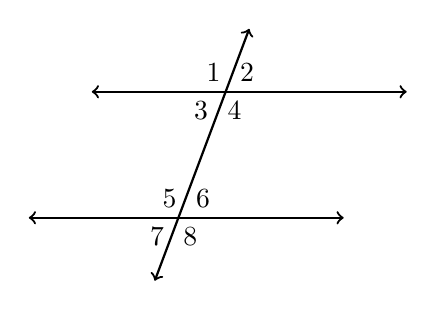
\begin{tikzpicture}[scale=0.8]
      \draw [<->, thick] (3,2)--(8,2);
      \draw [<->, thick] (2,0)--(7,0);
      \draw [<->, thick] (4,-1)--(5.5,3);
      \node at (4.5,0.3) [left]{$5$};
      \node at (4.5,0.3) [right]{$6$};
      \node at (4.3,-0.3) [left]{$7$};
      \node at (4.3,-0.3) [right]{$8$};
      \node at (5.2,2) [above left]{$1$};
      \node at (5.2,2) [above right]{$2$};
      \node at (5,2) [below left]{$3$};
      \node at (5,2) [below right]{$4$};
    \end{tikzpicture}
  \end{multicols}
  
\newpage
\item Given two parallel lines and a transversal, with $m\angle 4 = 3x$ and $m\angle 5 = x + 70$. \\ Write an equation, then solve for $x$.
\begin{flushright}
  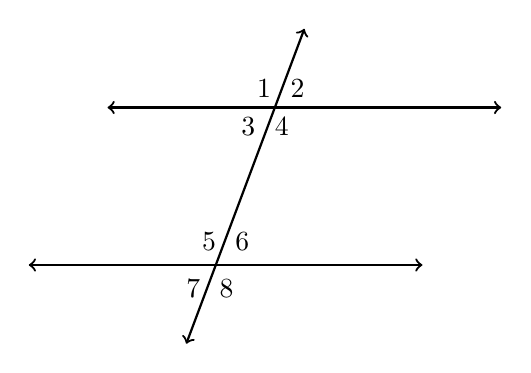
\begin{tikzpicture}[scale=1]
    \draw [<->, thick] (3,2)--(8,2);
    \draw [<->, thick] (2,0)--(7,0);
    \draw [<->, thick] (4,-1)--(5.5,3);
    \node at (4.5,0.3) [left]{$5$};
    \node at (4.5,0.3) [right]{$6$};
    \node at (4.3,-0.3) [left]{$7$};
    \node at (4.3,-0.3) [right]{$8$};
    \node at (5.2,2) [above left]{$1$};
    \node at (5.2,2) [above right]{$2$};
    \node at (5,2) [below left]{$3$};
    \node at (5,2) [below right]{$4$};
  \end{tikzpicture}
\end{flushright}

\newpage
\item Two parallel lines intersect a transversal. Given corresponding angles  $m\angle 1 = 4.4x - 63$ and $m\angle 2 = 2.8x+9$, find the measure of $\angle 1$. 
  \begin{flushright}
    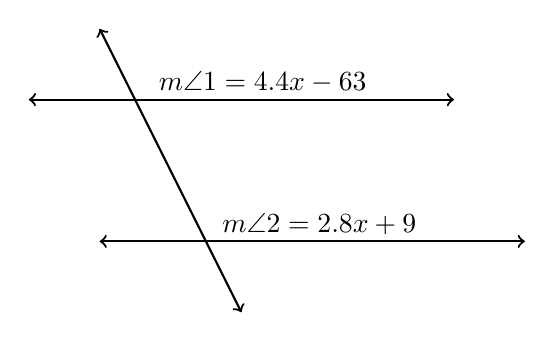
\begin{tikzpicture}[scale=0.9]
      \draw [<->, thick] (3,0)--(9,0);
      \draw [<->, thick] (2,2)--(8,2);
      \draw [<->, thick] (5,-1)--(3,3);
      %\draw [<->, thick] (11,-1)--(9,3);
      %\node at (4, 1.7){$1$};
      \node at (5.3, 2.25){$m\angle 1 = 4.4x - 63$};
      \node at (6.1, 0.25){$m\angle 2 = 2.8x+9$};
      %\node at (10, 0.25){$3$};
    \end{tikzpicture}
    \end{flushright}

\newpage
\item Given parallel lines $\overleftrightarrow{AB} \parallel \overleftrightarrow{CDE}$ with $\overline{AC} \cong \overline{CD}$. If $m\angle BAD=80$ find $m\angle ACD$.
  \begin{flushright}
  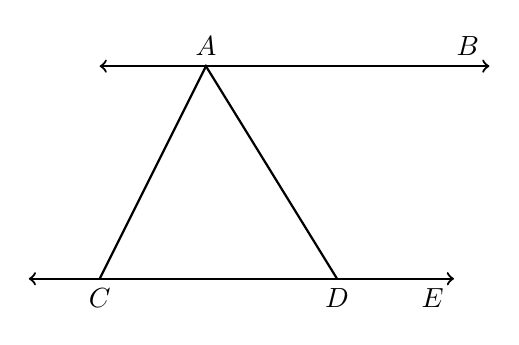
\begin{tikzpicture}[scale=0.9]
    \draw [<->, thick] (1,3)--(6.5,3) node[above left]{$B$};
    \draw [<->, thick] (0,0)--
      (5,0)--
      (6,0) node[below left]{$E$};
    \draw [-, thick] (1,0) node[below]{$C$}--
      (2.5,3) node[above]{$A$}--
      (4.35,0) node[below]{$D$};
  \end{tikzpicture}
  \end{flushright} \vspace{1cm}

\newpage
\item Two parallel lines intersect a second set of parallel lines. Given $m\angle 2 = 2.8x+9$ and $m\angle 4 = 4.4x - 63$, find the measure of $\angle 1$. 
  \begin{flushright}
    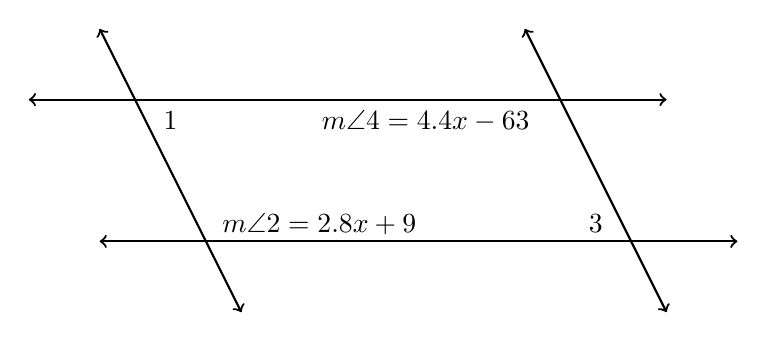
\begin{tikzpicture}[scale=0.9]
      \draw [<->, thick] (3,0)--(12,0);
      \draw [<->, thick] (2,2)--(11,2);
      \draw [<->, thick] (5,-1)--(3,3);
      \draw [<->, thick] (11,-1)--(9,3);
      \node at (4, 1.7){$1$};
      \node at (6.1, 0.25){$m\angle 2 = 2.8x+9$};
      \node at (10, 0.25){$3$};
      \node at (7.6, 1.7){$m\angle 4 = 4.4x - 63$};
    \end{tikzpicture}
    \end{flushright}
    
\end{enumerate}
\end{document}